\documentclass{beamer}

\usepackage{pgf,pdfpages}
\usepackage{listings}
%\usepackage{adjustbox}
\usepackage{graphicx} % http://tex.stackexchange.com/questions/38177/including-large-tables-in-a-beamer-frame

\usepackage[T1]{fontenc}
\usepackage{cmap}
\usepackage[utf8]{inputenc}
\lstset{breakatwhitespace,
    language=C++,
    columns=fullflexible,
    keepspaces,
    breaklines,
    tabsize=3,
    showstringspaces=false,
extendedchars=true}

\mode<presentation>
{
    %\usetheme{bunsen}
    \usetheme{Madrid}
    \setbeamercovered{transparent}
    \setbeamertemplate{items}[circle]
}

% suppress navigation bar
\beamertemplatenavigationsymbolsempty

\usefonttheme[onlymath]{serif}
\setbeamerfont{frametitle}{size=\LARGE,series=\bfseries}

\defbeamertemplate{enumerate item}{mycircle}
{
    \begin{pgfpicture}{0ex}{0ex}{1.5ex}{0ex}
        \pgfbox[center,base]{\insertenumlabel.}
    \end{pgfpicture}
}
[action]
{\setbeamerfont{item projected}{size=\scriptsize}}
\setbeamertemplate{enumerate item}[mycircle]

%% SPACING BETWEEN ITEMS FOR BEAMER
%% following lets me add length between items
%% http://tex.stackexchange.com/questions/16793/global-setting-of-spacing-between-items-in-itemize-environment-for-beamer
% \let\oldframe\frame
% \renewcommand{\frame}{
% \oldframe
% \let\olditemize\itemize
% %%\renewcommand\itemize{\olditemize\addtolength{\itemsep}{0.5\baselineskip}}
% \renewcommand\itemize{\olditemize\addtolength{\parskip}{0.5\baselineskip}} %% this affects nested list (itemize) as well
% }
\newlength{\wideitemsep}
\setlength{\wideitemsep}{\itemsep}
\addtolength{\wideitemsep}{0.5\baselineskip}
\let\olditem\item
\renewcommand{\item}{\setlength{\itemsep}{\wideitemsep}\olditem}
%%\usepackage{enumitem} %% traditional way to modify listing (itemize and enumerate) properties...but beamer has its own definition
%% NESTED LISTS
%% http://tex.stackexchange.com/questions/20654/length-between-nested-lists
\setbeamertemplate{itemize/enumerate subbody begin}{\vspace{0.5\baselineskip}}
\setbeamertemplate{itemize/enumerate subbody end}{\vspace{0.5\baselineskip}}
%% MORE OPTIONS http://tex.stackexchange.com/questions/11168/change-bullet-style-formatting-in-beamer

\title{Sega Game Gear on a Chip}
\author{Max Thrun | Samir Silbak}
\institute{University of Cincinnati}
\date{Fall 2012}

\begin{document}

\maketitle

%
% background for the rest of the slides
%
%\setbeamertemplate{background}
%{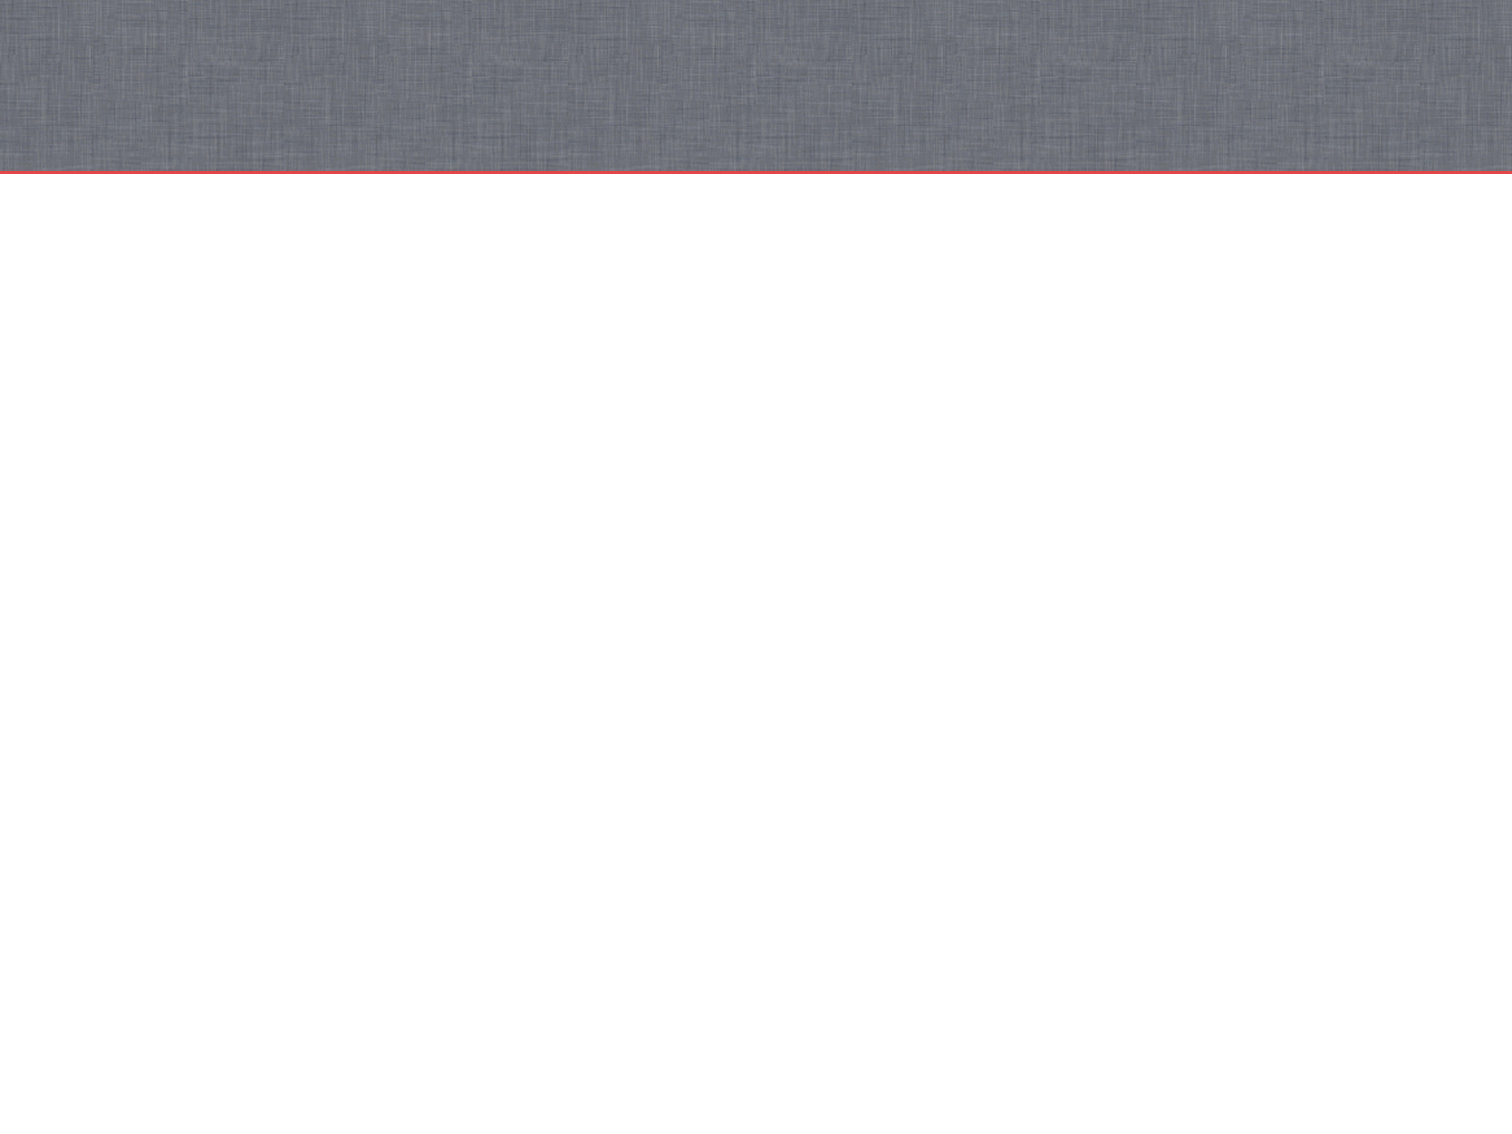
\includegraphics[width=\paperwidth,height=\paperheight]{slide_bg.png}}
%\setbeamertemplate{footline}[bunsentheme]

\section{Agenda}
\begin{frame}
\frametitle{Agenda}
    \begin{itemize}
        \item Problem Description
        \item Design Process
        \item Requirements/Assessment Metrics/Test Plan
        \item Design Overview
        \item Project Limitations
    \end{itemize}
\end{frame}

\section{Problem Description}
\begin{frame}
    \frametitle{Problem Description}
    \begin{center}
        \Large
        Reimplement all the digital components of \\a legacy computer system in a FPGA
    \end{center}
\end{frame}

\begin{frame}
    \frametitle{Problem Description}

    \begin{columns}[c]
        \column{0.6\textwidth}
            Why?
            \begin{itemize}
                \item<2-> \textbf{Maintainability} - You can no longer buy parts to service legacy computer systems
                \item<3-> \textbf{Upgradability} - Reimplementation gives an opportunity to add additional features
                \item<4-> \textbf{Portability} - Do not need all the original big clunky hardware. Reimplementation can
                    be embedded in new designs
            \end{itemize}

        \column{0.4\textwidth}
            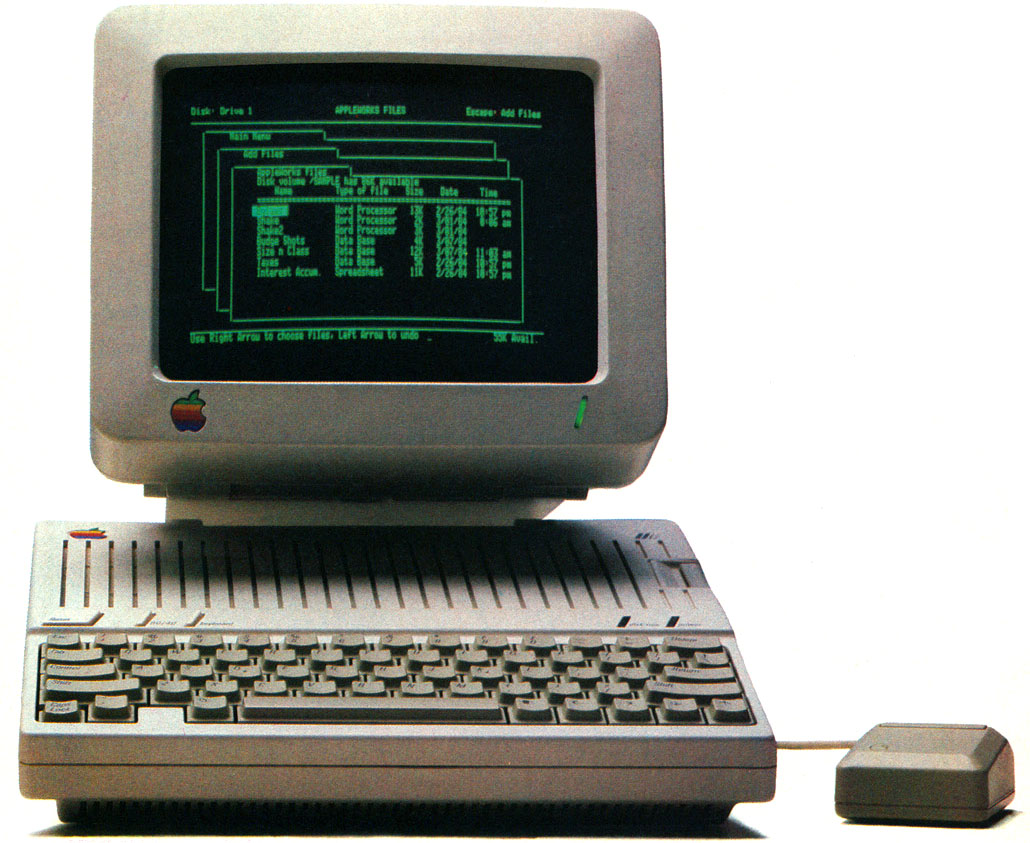
\includegraphics[width=\textwidth]{../images/apple_2.jpg}
    \end{columns}
\end{frame}

\section{Design Process}
\begin{frame}
    \frametitle{Design Process}
    \begin{center}
        WHY?
    \end{center}
\end{frame}

\section{Requirements/Assessment Metrics/Test Plan}
\begin{frame}
    \frametitle{Requirements/Ass. Metrics/Test Plan}
    \begin{enumerate}
        \item<1-> Break down system components according to the original system architecture
        \item<2-> Implement each component to match the original functionality described by official and
            non official documents
        \item<3-> Test each components functionality against the actual hardware (in our case an emulator)
        \item<4-> Tie components together in a way that is better suited toward FPGA technology (\emph{E.g.} avoid tri-state buses)
    \end{enumerate}
\end{frame}

%\begin{frame}[fragile] % fragile for lstlisting
\begin{frame}
    \frametitle{Requirements/Ass. Metrics/Test Plan}
    In order to test the operation of the z80, and basic functionality of the VDP,
    custom ROMs were developed. Using the Small Device C Compiler (SDCC)
    \cite{SDCC} we are able to write programs that exercises various functionality
    of the system.

    We found SDCC extremely easy to setup and get working. The only thing we needed
    to modify was the stack pointer location in the C Runtime file (crt0.s). The
    default stack pointer location is set to \texttt{0xFFFF} but the top most RAM
    address on the Game Gear is \texttt{0xDFFF}. Setting up IO is as easy as
    specifying a special function register at a given IO port. An example showing
    how to write data to the VDP data port (0xBE) is shown below.
\end{frame}

\defverbatim[colored]\lst{%
    \begin{lstlisting}[captionpos=b, caption=VDP Data Write]
        __sfr __at (0xBE) vdp_data;
        int main() {
            vdp_data = 0x38;    // write 0x38 to VDP data port
            while (1) {}
            return 0;
        }
    \end{lstlisting}}

    \begin{frame}
        \frametitle{Requirements/Ass. Metrics/Test Plan}
        \lst
    \end{frame}

    \begin{frame}
        \frametitle{Requirements/Ass. Metrics/Test Plan}
        \begin{center}
            We ended up building a small GG library with the following functions:
        \end{center}
    \end{frame}

\defverbatim[colored]\lst{%
    \begin{lstlisting}[captionpos=b, caption=Game Gear Library Functions]
        void vdp_write_control(uint8_t value);
        void vdp_write_data(uint8_t value);
        void vdp_set_register(uint8_t reg, uint8_t value);
        void vdp_set_vram_addr(uint16_t addr);
        void vdp_set_palette(uint8_t id, uint16_t color);
        void set_pattern_fill(uint16_t id, uint8_t color);
        void set_tile_to_pattern(uint8_t x, uint8_t y, uint16_t pattern);
        void delay(uint16_t x);
        void set_debug(uint8_t x);
    \end{lstlisting}}

    \begin{frame}
        \frametitle{Requirements/Ass. Metrics/Test Plan}
        \lst
    \end{frame}

\begin{frame}
    \frametitle{Requirements/Ass. Metrics/Test Plan}
    With this library in place it is easy to to perform operations such as setting
    up the color palette:
\end{frame}

\defverbatim[colored]\lst{%
    \begin{lstlisting}[captionpos=b, caption=Color Palette Test ROM]
        #include <gg.h>
        int main() {
            // set register 1 bit 6 to enable display
            vdp_set_register(1, (1<<6));
            // set first color palette entry to gray
            vdp_set_palette(0, 0x0CCC);
            while (1) {}
            return 0;
        }
    \end{lstlisting}}

    \begin{frame}
        \frametitle{Requirements/Ass. Metrics/Test Plan}
        \lst
    \end{frame}

    \begin{frame}
        \frametitle{Requirements/Ass. Metrics/Test Plan}
        In order to test the operation of the VDP background generator a separate test
        project used which only consists of the background generator, VRAM, VGA timing
        generator, and a UART interface.

        Games are run using the open-source Osmose Sega Emulator \cite{osmose}. When
        the game reaches a screen that we want to test on the FPGA we dump the VRAM and
        CRAM using Osmoses built in debugger. We then use programs, written in C, that
        read the VRAM dump and generate images of the color palette, all 512 background
        tiles, and the final screen rendering.  These programs serve a dual purpose
        allowing us to both confirm our understanding of how the background image is
        generated and also that our VRAM dump is valid. The images below show example
        output from these three programs.
    \end{frame}
    %\begin{frame}
    %    \frametitle{Requirements/Ass. Metrics/Test Plan}
    %\begin{columns}[c]
    %    \column{0.45\textwidth}
    %    
\includegraphics[width=\textwidth]{../images/palette.png}
    %    %\caption{Color Palette}
    %    \column{0.45\textwidth}
    %    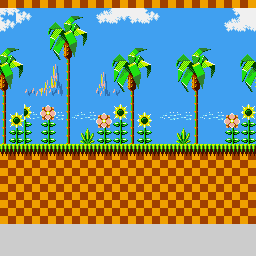
\includegraphics[width=\textwidth]{../images/screen.png}
    %    %\caption{Complete Screen Render}
    %\end{columns}
%\end{frame}

\begin{frame}
    \frametitle{Requirements/Ass. Metrics/Test Plan}
    \begin{figure}[H]
        \centering
        \begin{minipage}[H]{0.45\linewidth}
            \centering
            
\includegraphics[width=\textwidth]{../images/palette.png}
            \caption{Color Palette}
            \label{fig:palette}
        \end{minipage}
        \hfill
        \begin{minipage}[H]{0.45\linewidth}
            \centering
            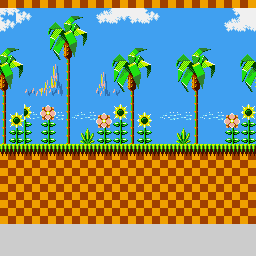
\includegraphics[width=\textwidth]{../images/screen.png}
            \caption{Complete Screen Render}
            \label{fig:screen}
        \end{minipage}
    \end{figure}
\end{frame}

\begin{frame}
    \frametitle{Requirements/Ass. Metrics/Test Plan}
    \begin{figure}[H]
        \centering
        \begin{minipage}[H]{0.8\linewidth}
            \centering
            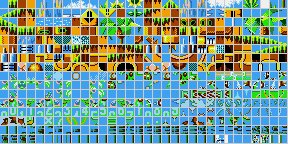
\includegraphics[width=\textwidth]{../images/tiles.png}
            \caption{All 512 Tiles}
            \label{fig:tiles}
        \end{minipage}
    \end{figure}
    \vfill
    %\begin{columns}[c]
    %    \column{0.8\textwidth}
    %    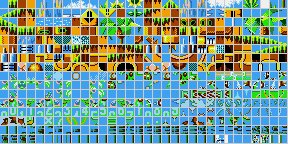
\includegraphics[width=\textwidth]{../images/tiles.png}
    %    \caption{All 512 Tiles}
    %\end{columns}
\end{frame}

\begin{frame}
    \frametitle{Requirements/Ass. Metrics/Test Plan}
        %\adjustbox{max height=\dimexpr\textheight-5.5cm\relax,
                       %max width=0.1mm}{
        \resizebox{\linewidth}{!}{% Resize table to fit within \linewidth horizontally
        \begin{tabular}{|c|c|c|c|c|c|}
            \hline
            Function    & Requirement Spec.     & Design Verified?  & Test Protocol     & Signature     \\ \hline
            6           & test                  &    test           &    test           &    test       \\
            \hline
        \end{tabular}}
\end{frame}

\section{Design Overview}
\begin{frame}
    \frametitle{Design Overview}
    \begin{columns}[c]
        %\column{0.8\textwidth}
        \column{0.3\textwidth}
        Black Box Diagram
    \end{columns}
    \begin{center}
        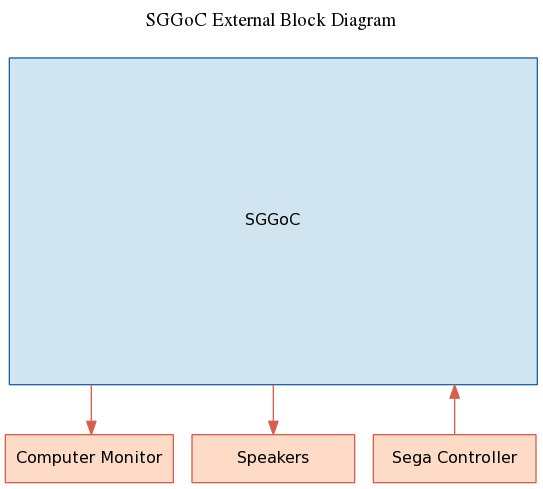
\includegraphics[scale=0.4]{../block_diagrams/block_diagram_external.png}
    \end{center}
\end{frame}

\begin{frame}
    \frametitle{Design Overview}
    \begin{columns}[c]
        %\column{1.0\textwidth}
        \column{0.4\textwidth}
        \vspace{-0.8cm}
        Internal Functional Diagram
    \end{columns}
    \begin{center}
        %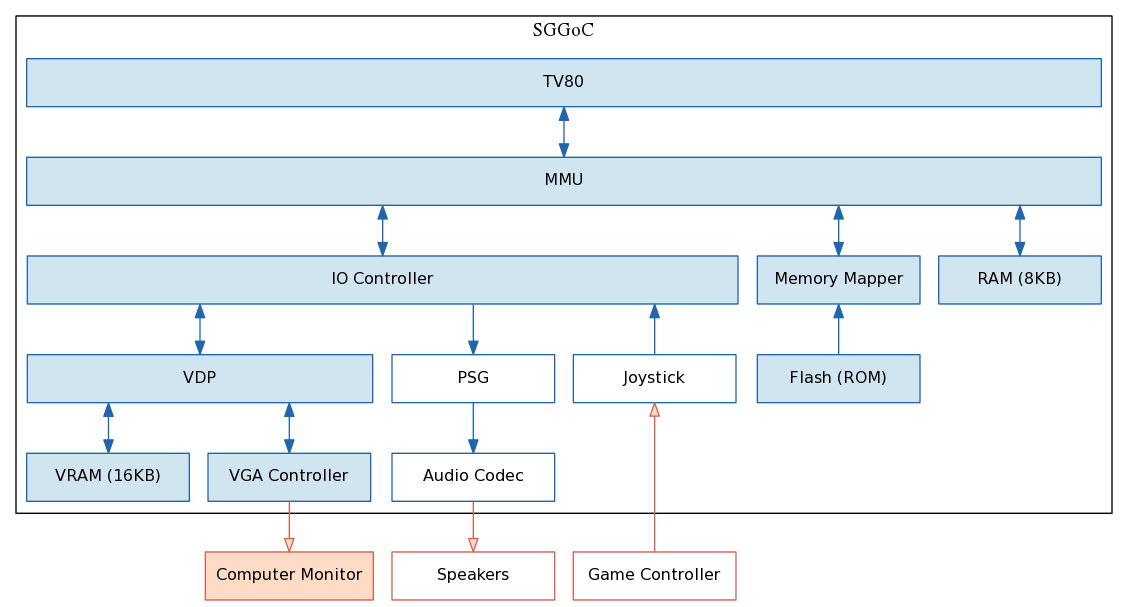
\includegraphics[width=\textwidth]{../block_diagrams/block_diagram_internal_implemented.png}
        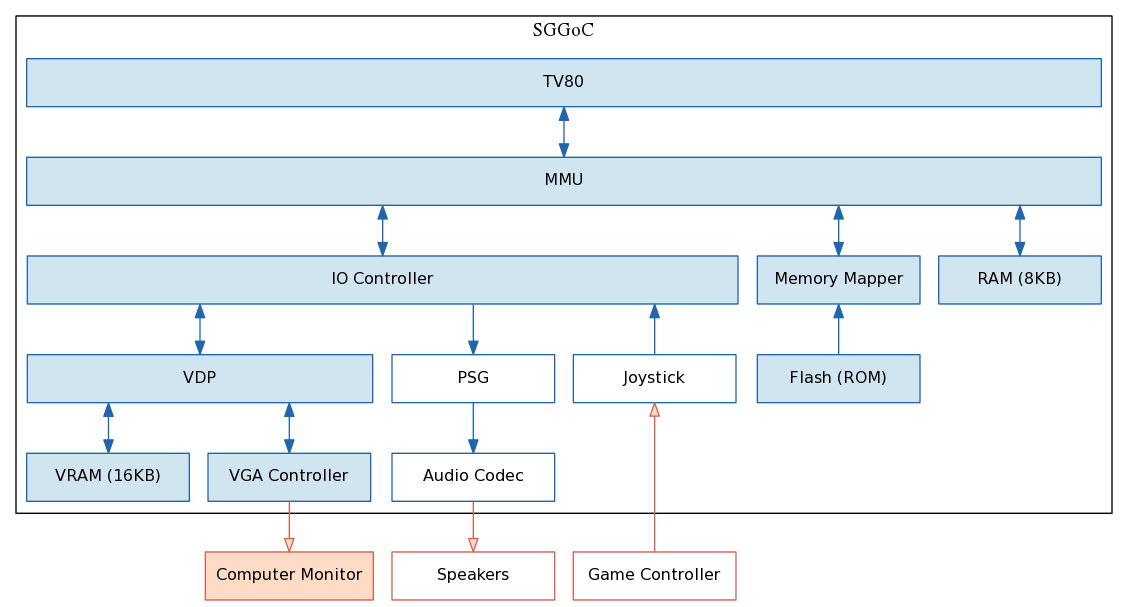
\includegraphics[scale=0.3]{../block_diagrams/block_diagram_internal_implemented.png}
    \end{center}
\end{frame}

\begin{frame}
    \frametitle{Design Overview}
    \begin{columns}[c]
        \column{0.45\textwidth}
        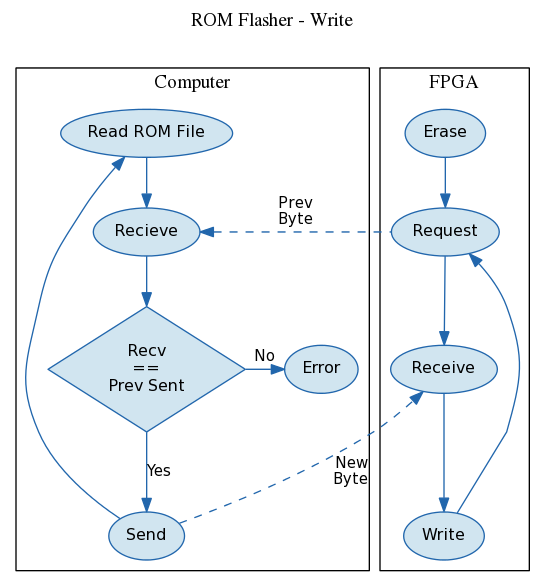
\includegraphics[width=\textwidth]{../../fpga/rom_flasher/doc/block_diagram_write.png}
        \column{0.45\textwidth}
        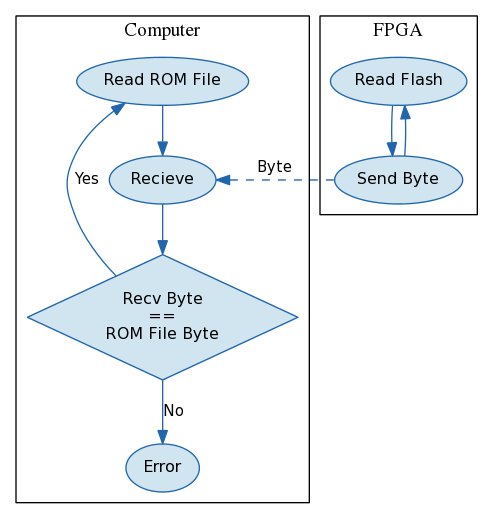
\includegraphics[width=\textwidth]{../../fpga/rom_flasher/doc/block_diagram_read.png}
    \end{columns}
\end{frame}

\section{Project Limitations}
\begin{frame}
    \frametitle{Project Limitations}
    Game Gear is hard to test/verify
    \begin{itemize}
            \olditem<2-> Its only output is video (no UART, JTAG, etc..)
            \olditem<3-> Most documentation is 3rd party
    \end{itemize}
    \vspace{0.25cm}
    \onslide<4->{Our strategy:}
    \begin{enumerate}
        \olditem<5-> Use an emulator to watch memory fetches and get memory dumps
        \olditem<6-> Initialize our RAMs with these dumps and verify we achieve the same visual output
        \olditem<7-> Watch instruction fetches with a logic analyzer and see if they match the emulator
    \end{enumerate}
    \vspace{0.25cm}
    \onslide<8->{Could replace emulator with a logic/bus analyzer connected to the original hardware}
\end{frame}

\begin{frame}
\frametitle{}
    \begin{center}
        \Huge
        Questions?
    \end{center}
\end{frame}

\newpage

\section{Bibliography}
\begin{frame}
    \frametitle{References}
    \begin{thebibliography}{9}
    %\bibitem{gg} \url{http://mo5.com/musee-machines-gamegear.html}
    %\bibitem{gg_cart} \url{http://www.magisterrex.com/prodimages/EccoDolphinGameGear-h450.png}
    %\bibitem{gg_cart_pcb} \url{http://www.smspower.org/Development/SMSPagingChips}
    %\bibitem{mapper} \url{http://www.smspower.org/Development/Mappers}
    %\bibitem{flash_core} \url{ftp://ftp.altera.com/up/pub/flash/altera_up_flash_memory.zip}
    %\bibitem{tv80} \url{http://opencores.org/project,tv80}
    %\bibitem{mem_map_table} \url{http://code.google.com/p/bizhawk/source/browse/trunk/BizHawk.Emulation/Consoles/Sega/SMS/MemoryMap.Sega.cs}
    %\bibitem{VDP} \url{http://www.smspower.org/uploads/Development/msvdp-20021112.txt?sid=c8bdf72dd28a0a34eeedf5f7742ca62a}
            \bibitem{osmose} \url{http://bcz.asterope.fr/osmose.htm}
    %\bibitem{ieeeverilog} \url{http://ieeexplore.ieee.org/stamp/stamp.jsp?arnumber=00954909}
    %\bibitem{gpl} \url{http://www.gnu.org/licenses/gpl.html}
            \bibitem{SDCC} \url{http://sdcc.sourceforge.net/}
    \end{thebibliography}
\end{frame}

\end{document}
